% \documentclass[8pt,xcolor=pdftex,table,handout]{beamer}

\documentclass[8pt,xcolor=pdftex,table]{beamer}
\include{preambule_beamer}

\usepackage{listings}

% \usepackage{amsmath}
% \usepackage{unicode-math}
% \setmathfont{Fira Math}


% \usepackage{animate}

% ------------------------------------------- %

\graphicspath{{Figures/} {Figures/Logos/} {../Figures/}}
% \graphicspath{{../Figures/} {../Figures/Logos/}}

\title[]{\vspace{22mm}Formation \alert{Ingénieur Machine Learning}\\\vspace{6mm}Projet:\\\alert{Classez automatiquement des questions}}
\date[]{\alert{XX} Mai 2023\\\vspace{18mm}\\\tit{thomas.durandtexte@protonmail.com}}


\titlegraphic{\hfill
\def\arraystretch{.1}%  1 is the default, change whatever you need
	\begin{tabular}{ >{\centering}m{7mm} m{39mm} }
		
\includegraphics[height=7mm]{Logo_OpenClassrooms.png }
		&
		\Large{\textbf{OPENCLASSROOMS}}
	\end{tabular}
}

% \definecolor{clrData}{rgb}{0.9,0.5,0}

\tikzstyle{box_style00}=[draw, rounded corners,anchor=center,text centered,text=white]
% \tikzstyle{diagram0}=[box_style00, text width=22mm, minimum height=12mm]
% \tikzstyle{dataset}=[box_style00,diagram0, fill=blue]
% \tikzstyle{filtrage}=[box_style00,diagram0, fill=red!80]
% \tikzstyle{doublons}=[box_style00,diagram0, fill=magenta!80]
% \tikzstyle{datavoisins}=[box_style00,diagram0, fill=cyan!80]
% \tikzstyle{outliers}=[box_style00,diagram0, fill=magenta!80]

% \includeonlyframes{CCL,Perspectives}



\begin{document}
% ------------------------------------------- %

\begin{frame}
	\titlepage{}
\end{frame}


\section{CONTEXTE}


\begin{frame}[t, label=contexte]
	\vspace{0mm}
	\begin{tikzpicture}
		\linespread{1}% <--- locally defined vertical line spacing in nodes
		\draw[clrBorders] (0,0) rectangle (\txw,\txh) ;
		\nodePageNumber

		\onlystyle<2->{removed}{myShaded}
		\node[box_style00, text width = 40mm, removed] at (0.5\txw,80mm)
			{Aide à la communauté stackoverflow / stackexchange} ;

		\visible<2->{
		\node[box_style00, minimum height = 15mm] at (0.3\txw, 50mm) (Q)
			{Questions posées} ;
		}
		\visible<3->{
			\node[box_style00, minimum height = 15mm, text width=20mm] at (0.7\txw, 50mm) (T)
				{Plusieurs tags \only<-4>{associés\phantom{s}}\only<5>{\alert{suggérés}} à chaque questions} ;
			\draw[myarrow] (T) -- (Q) ;
		}

		\visible<4->{
			\node[box_style00] at (0.5\txw, 30mm) (P)
				{Predicteur} ;
			\draw[myarrow] (Q) |- (P) ;
		}
		\visible<5>{
			\draw[myarrow, myOrng] (P) -| (T) ;
		}
	\end{tikzpicture}
\end{frame}

\subsection{Base de données}
\begin{frame}[t, label=BaseDonnees]
	\vspace{0mm}
	\begin{tikzpicture}
		\linespread{1}% <--- locally defined vertical line spacing in nodes
		\draw[clrBorders] (0,0) rectangle (\txw,\txh) ;
		\nodePageNumber

		\node at (\midX,80mm) {Requête SQL} ;

		\node at (\midX,\midY) {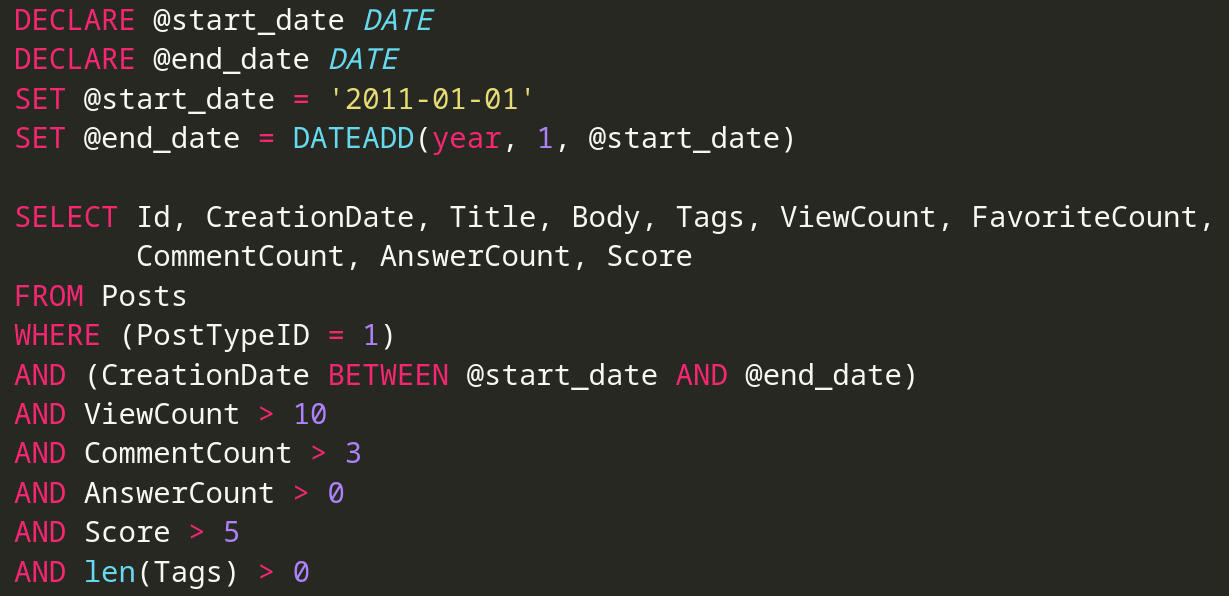
\includegraphics[width=90mm]{SQL_querry.png}} ;

		\only<2>{
			\draw[rounded corners, myOrng, thick] (30mm,55.5mm) rectangle (68mm,62mm) ;
			\node[myOrng, text width=30mm, text centered] at (83mm,58.5mm) {1 requête par année jusqu'en 2022 inclus} ;
		}

		\only<3>{
			\begin{scope}[yshift=44.5mm]
				\draw[rounded corners, myOrng, thick] (9mm,-3mm) rectangle (40mm,3mm) ;
				\node[myOrng, text width=30mm, text centered, font=\bfseries] at (50mm,0) {Questions} ;
			\end{scope}
		}

		\only<4>{
			\begin{scope}[yshift=33mm]
				\draw[rounded corners, myOrng, thick] (9mm,-9mm) rectangle (80mm,9mm) ;
				\node[myOrng, text width=30mm, text centered, font=\bfseries] at (55mm,0) {Contraintes pour la "qualité" des données} ;
			\end{scope}
		}

		\only<5>{
			\node (B) at (20mm, 24.5mm) {} ;
			\node (A) at (\midX,12mm) {275 325 questions} ;
			\draw[myarrow] (B) |- (A) ;
		}
	\end{tikzpicture}
\end{frame}


\subsection{Protocole}
\begin{frame}[t, label=protocol]
	\vspace{0mm}
	\begin{tikzpicture}
		\linespread{1}% <--- locally defined vertical line spacing in nodes
		\draw[clrBorders] (0,0) rectangle (\txw,\txh) ;
		\nodePageNumber


		\onlystyle<4->{shd1}{myShaded}
		\onlystyle<5->{shd2}{myShaded}
		\onlystyle<6->{shd3}{myShaded}
		\onlystyle<7->{shd4}{myShaded}
		\onlystyle<7->{showed4}{myFnt}

		\begin{scope}[xshift=35mm]
			\node[box_style00,shd1] (Data) at (0mm,80mm) {Base de données} ;

			\visible<2->{
				\node[box_style00, text width=20mm, shd2] (Text) at (-15mm, 60mm) {Données {\color<-4>{myOrng}\textbf{textuelles}}} ;
				\draw[myarrow,shd1] (Data) -- ++(0,-9mm) -| (Text) ;
			}
			\visible<3->{
				\node[box_style00,shd3, text width=20mm] (Tags) at (15mm, 60mm) {Liste de {\color<-5>{myOrng}\textbf{tags}} par question} ;
				\draw[myarrow,shd1] (Data) -- ++(0,-9mm) -| (Tags) ;
			}

			\visible<4->{
				\node[box_style00,shd4, text width = 18mm] (Encode) at (-15mm, 40mm) {Nettoyage\\\&\\encodage} ;
				\draw[myarrow,shd2] (Text) -- (Encode) ;
			}

			\visible<5->{
				\node[box_style00,shd3,showed4, text width=50mm] (Model) at (0, 20mm) {Entrainement d'un classifieur\\méthode "OneVsRest"} ;
				\draw[myarrow,shd3] (Encode) -- ++(0, -16.3mm) ;
				\draw[myarrow,shd3] (Tags) -- ++(0, -36.3mm) ;
			}

		\end{scope}

		\visible<6->{
			\node[shd4] at (80mm,40mm) {Essais de différents encodeurs} ;
		}

		\visible<7->{
			\node[text width=40mm, text centered] at (83mm,20mm) {Essais de\\différents classifieurs} ;
		}
	\end{tikzpicture}
\end{frame}


\section{EXPLORATION DES DONNÉES}

\subsection{Valeurs manquantes}
\begin{frame}[t, label=MissingValues]
	\vspace{0mm}
	\begin{tikzpicture}
		\linespread{1}% <--- locally defined vertical line spacing in nodes
		\draw[clrBorders] (0,0) rectangle (\txw,\txh) ;
		\nodePageNumber

		\node at (\midX,\midY) {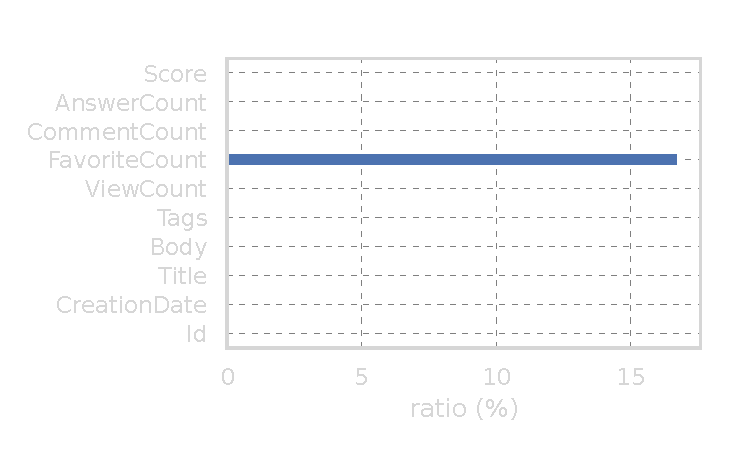
\includegraphics[width=80mm]{ratio_isnull.pdf}} ;

		\node<2> at (\midX,15mm) {Mise à part le \alert{FavoriteCount}, les \alert{données} sont \alert{complètes}} ;
	\end{tikzpicture}
\end{frame}


\subsection{Questions}

\begin{frame}[t, label=QPerYear]
	\vspace{0mm}
	\begin{tikzpicture}
		\linespread{1}% <--- locally defined vertical line spacing in nodes
		\draw[clrBorders] (0,0) rectangle (\txw,\txh) ;
		\nodePageNumber

		\node at (\midX,\midY) {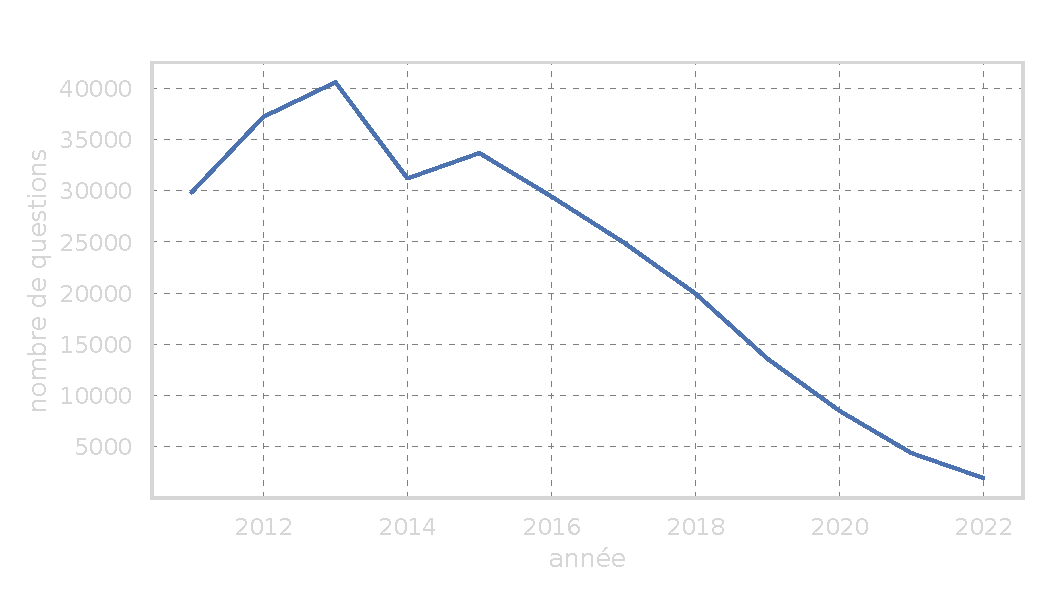
\includegraphics[width=90mm]{q_per_y.pdf}} ;

		\node<2> at (\midX, 15mm) {\alert{Diminution conséquente} avec le temps (utilisation de l'existant, AI, ...)} ;
	\end{tikzpicture}
\end{frame}


\begin{frame}[t, label=QlenPerYear]
	\vspace{0mm}
	\begin{tikzpicture}
		\linespread{1}% <--- locally defined vertical line spacing in nodes
		\draw[clrBorders] (0,0) rectangle (\txw,\txh) ;
		\nodePageNumber

		\only<1-2>{
			\node at (\midX,\midY) {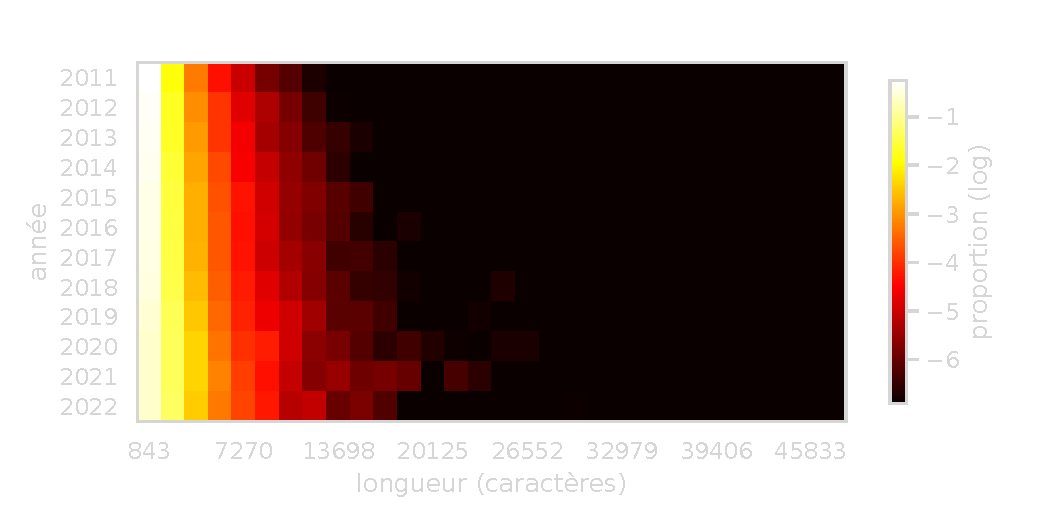
\includegraphics[width=90mm]{arr_length_per_year_body.pdf}} ;
		}

		\node<2> at (\midX, 15mm) {\alert{Longueur} des corps de texte \alert{relativement constante} dans le temps} ;

		\only<3-4>{
			\node at (\midX,\midY) {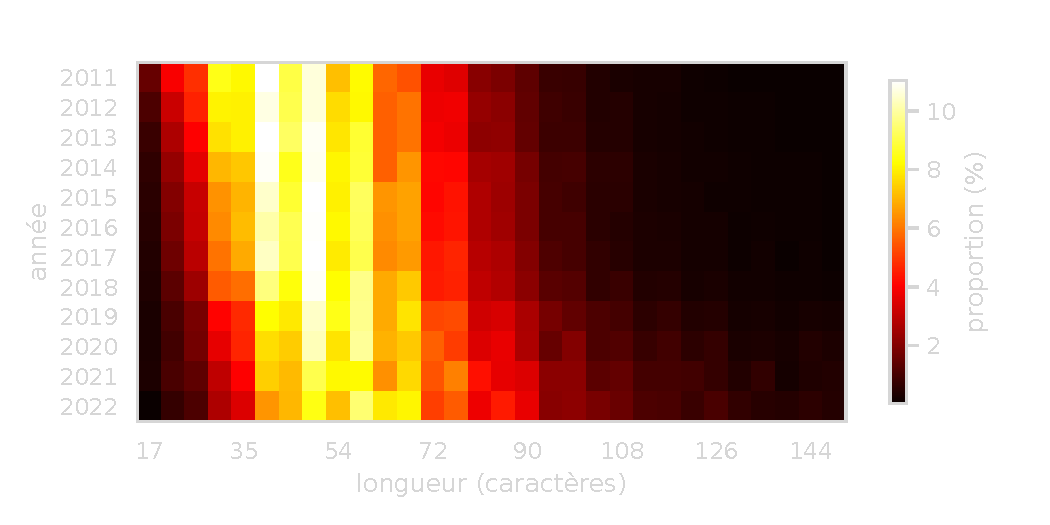
\includegraphics[width=90mm]{arr_length_per_year_title.pdf}} ;
		}
		\node<4> at (\midX, 15mm) {\alert{Allongement} des \alert{titres} des questions dans le temps} ;

	\end{tikzpicture}
\end{frame}


\subsection{Tags}

\begin{frame}[t, label=TagsPerY]
	\vspace{0mm}
	\begin{tikzpicture}
		\linespread{1}% <--- locally defined vertical line spacing in nodes
		\draw[clrBorders] (0,0) rectangle (\txw,\txh) ;
		\nodePageNumber

		\node at (\midX,85mm) {Tags les plus présents en 2011 et 2022} ;
		\node at (\midX,\midY-5mm) {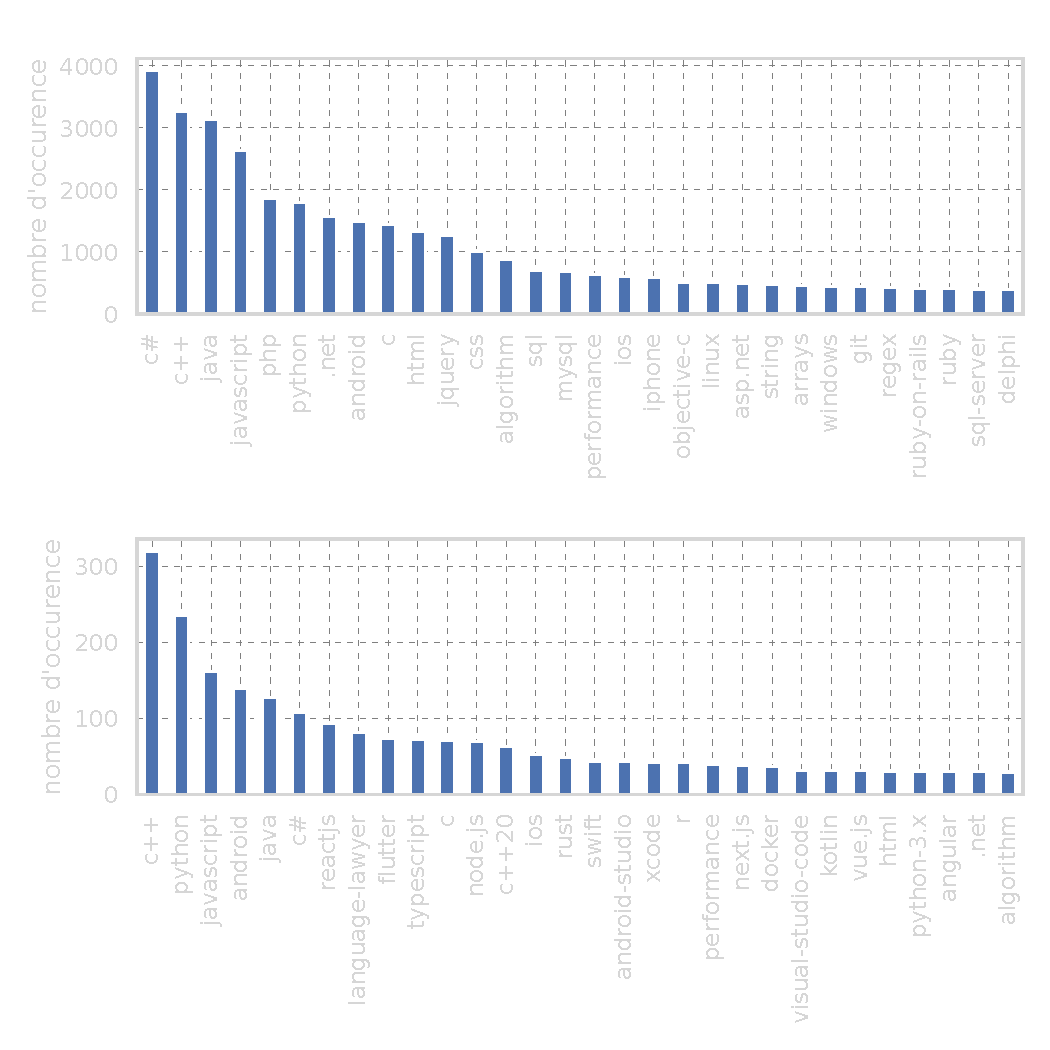
\includegraphics[width=80mm]{tags_per_y.pdf}} ;

		\node<2>[myOrng, font=\bfseries, text width=30mm, text centered] 
			at (\midX-15mm, 43mm) {Modification des sujets avec le temps} ;

	\end{tikzpicture}
\end{frame}


\begin{frame}[t, label=TagsMostUsed]
	\vspace{0mm}
	\begin{tikzpicture}
		\linespread{1}% <--- locally defined vertical line spacing in nodes
		\draw[clrBorders] (0,0) rectangle (\txw,\txh) ;
		\nodePageNumber

		\only<1>{
			\node at (\midX,75mm) {Estimation 2017 - 2023} ;
			\node at (\midX,\midY) {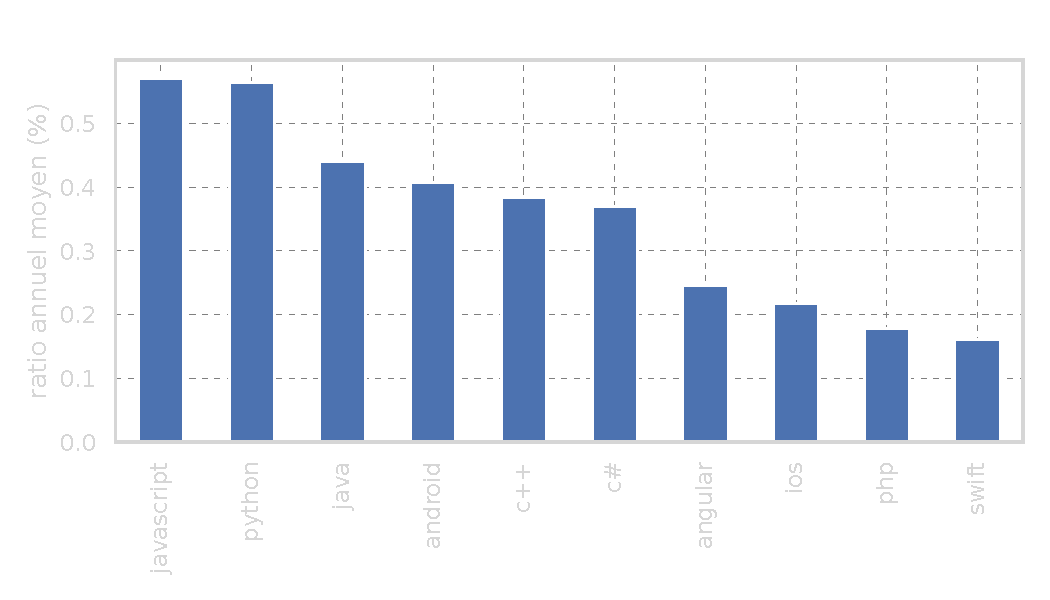
\includegraphics[width=90mm]{most_used_tags.pdf}} ;
		}
		\only<2->{
			\node at (\midX,\midY) {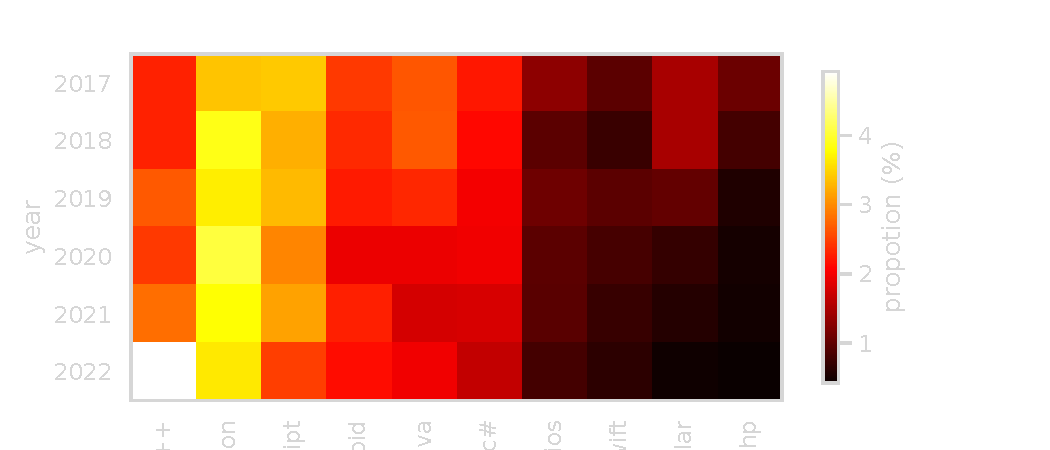
\includegraphics[width=90mm]{most_used_tags_per_year.pdf}} ;
		}
		\node<3> at (\midX, 15mm) {Les \alert{proportions varient} dans le temps} ;
	\end{tikzpicture}
\end{frame}

\begin{frame}[t, label=ProportionTagsInDataset]
	\vspace{0mm}
	\begin{tikzpicture}
		\linespread{1}% <--- locally defined vertical line spacing in nodes
		\draw[clrBorders] (0,0) rectangle (\txw,\txh) ;
		\nodePageNumber

		\node at (\midX,85mm) {\color<2->{myShaded} Pour cette analyse, \alert{10 tags} sont conservés} ;
		\node<2->[text centered, text width=100mm] at (\midX,75mm)
			{\color<3->{myShaded} Suppression des questions sans aucun des tags étudiés\\(275~325 $\rightarrow$ \alert{173~255 questions})} ;

		\node<3-> at (\midX,40mm) {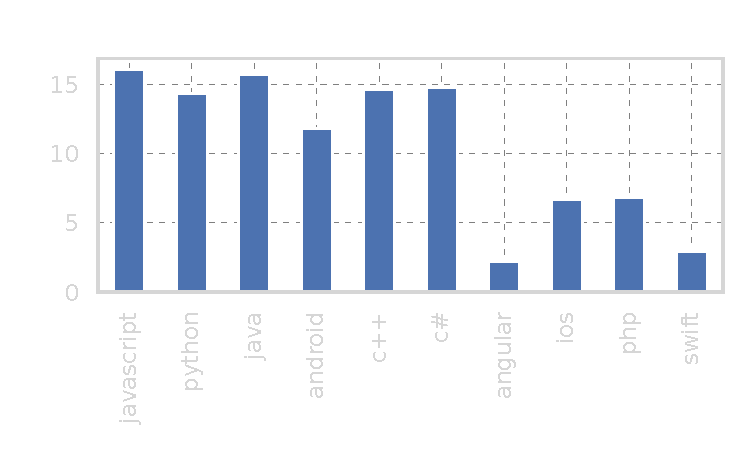
\includegraphics[width=80mm]{prop_tags.pdf}} ;

		\node<4> at (\midX,10mm) {Seulement \alert{10~441 questions} avec \alert{plus d'un des tags} sélectionnés} ;
	\end{tikzpicture}
\end{frame}


\subsection{Traitements}

\begin{frame}[t, label=Process]
	\vspace{0mm}
	\begin{tikzpicture}
		\linespread{1}% <--- locally defined vertical line spacing in nodes
		\draw[clrBorders] (0,0) rectangle (\txw,\txh) ;
		\nodePageNumber

		\onlystyle<2->{shd1}{myShaded}
		\node[shd1] at (\midX,80mm) {Chaîne de traitement des entrées} ;

		\begin{scope}[xshift=0.25*\txw, node distance=15mm]
			\node<2->[box_style00] (A) at (0,60mm) {Nettoyage} ;
			\node<4->[box_style00, below=of A] (B) {Tokenisation} ;
			\draw<4->[myarrow] (A) -- (B) ;
			\node<6->[box_style00, below=of B] (C) {Lemmatisation} ;
			\draw<6->[myarrow] (B) -- (C) ;

			\onlystyle<4->{shaded1}{myShaded}
			\node<3->[right=of A, text width=45mm, shaded1]
				{$\bullet$ Majuscules $\rightarrow$ minuscules~;\\$\bullet$ remplacement des contractions~;\\$\bullet$ suppression URL, html, non ascii, caractères spéciaux} ;

			\onlystyle<6->{shaded2}{myShaded}
			\node<5->[right=of B, shaded2, text width=45mm] {$\bullet$ Séparation des mots\\$\bullet$ Suppression des mots courants} ;

			\node<7->[right=of C, text width=44mm] {$\bullet$ Translation des mots vers leur forme canonique} ;
		\end{scope}

	\end{tikzpicture}
\end{frame}


\begin{frame}[t, label=ProcessExample]
	\vspace{0mm}
	\begin{tikzpicture}
		\linespread{1}% <--- locally defined vertical line spacing in nodes
		\draw[clrBorders] (0,0) rectangle (\txw,\txh) ;
		\nodePageNumber

		\onlystyle<2->{shd1}{myShaded}
		\node[shd1] at (\midX,85mm) {Exemple de traitement} ;

		\onlystyle<4->{shd2}{myShaded}
		\node<2->[shd2] at (\midX,75mm) {Entrée brute:} ;
		\node<3->[shd2] at (\midX,70mm) {$<$p$>$I've created a C\# WinForms application using VS2010...} ;

		\onlystyle<6->{shd3}{myShaded}
		\node<4->[shd3] at (\midX,60mm) {Entrée nettoyée:} ;
		\node<5->[shd3] at (\midX,55mm) {i have created a c\# winforms application using vs2010...} ;

		\onlystyle<8->{shd4}{myShaded}
		\node<6->[shd4] at (\midX,45mm) {Entrée tokenisée:} ;
		\node<7->[shd4] at (\midX,40mm) {'created', 'c\#', 'winforms', 'application', 'using', 'vs2010'...} ;

		\onlystyle<10->{shd5}{myShaded}
		\onlystyle<12->{hihgl}{myOrng}
		\node<8->[shd5, hihgl] at (\midX,30mm) {Entrée lemmatisée:} ;
		\node<9->[shd5, hihgl] at (\midX,25mm) {'create', 'c\#', 'winform', 'application', 'use', 'vs2010'...} ;

		\onlystyle<12->{shd6}{myShaded}
		\node<10->[shd6] at (\midX,15mm) {Entrée stemmatisée (example):} ;
		\node<11->[shd6] at (\midX,10mm) {'creat', 'c\#', 'winform', 'applic', 'use', 'vs2010'...} ;

		\begin{scope}[xshift=\midX, yshift=12.5mm]
			\fill<12> [
		   pattern={Lines[
					  distance=9mm,
					  angle=30,
					  line width=0.4mm,
					  xshift=13mm,
					 ]},
			pattern color=myOrng
		   ] (-33mm,-6mm) rectangle (+33mm,6mm);
		\end{scope}
	\end{tikzpicture}
\end{frame}





\section{ESSAIS DE MODÉLISATIONS}

\subsection{Méthode non supervisée : Latent Dirichlet Allocation}
\begin{frame}[t, label=LDA]
	\vspace{0mm}
	\begin{tikzpicture}
		\linespread{1}% <--- locally defined vertical line spacing in nodes
		\draw[clrBorders] (0,0) rectangle (\txw,\txh) ;
		\nodePageNumber

		\onlystyle<2->{shd1}{myShaded}
		\node[shd1] at (\midX,80mm) {Encodeur : TFIDF (1000 mots)} ;

		\node<2-> at (\midX,\midY) {\includegraphics<2->[width=90mm]{LDAvis.png}} ;

		\node<3>[myOrng] at (\midX,10mm) {À priori pas utilisable pour ce projet} ;

	\end{tikzpicture}
\end{frame}

\subsection{Quel classifieur ?}

\begin{frame}[t, label=Classifieurs]
	\vspace{0mm}
	\begin{tikzpicture}
		\linespread{1}% <--- locally defined vertical line spacing in nodes
		\draw[clrBorders] (0,0) rectangle (\txw,\txh) ;
		\nodePageNumber

		\onlystyle<2->{shd1}{myShaded}
		\node[shd1] at (\midX,80mm) {Encodeur : TFIDF (300 mots)} ;

		\onlystyle<9->{shd4}{myShaded}
		\begin{scope}[xshift=75mm]
			\node<8->[shd4] at (0,70mm) {Modèles non-explorés:} ;
			\node<9->[box_style00] at (0,55mm) {SVC: non convergeant} ;
			\node<10->[box_style00] at (0,40mm) {ExtraTrees: calculs très longs} ;
			\node<11->[text width=40mm, text centered] at (0,32mm)
				{Dans un \alert{contexte industriel}: \alert{calculs} effectués sur \alert{serveur}} ;
		\end{scope}

		\onlystyle<3->{shd2}{myShaded}
		\onlystyle<8->{shd3}{myShaded}
		\begin{scope}[xshift=30mm, yshift=75mm]
			\node<2->[shd2] at (0,-5mm) {Modèles explorés:} ;
			\foreach[count=\i, evaluate=\i as \ii using int(\i+2)] \x in {Logistic Regression, SGD Classifier, Multinomial NB, Perceptron, Passive Aggressive Classifier}
			{
				\node<\ii->[box_style00, shd3] at (0,-\i*12mm) {\x} ;
			}
			% \node at (0, 70mm) {} ;
			% \node at (0, 60mm) {} ;
			% \node at (0, 50mm) {} ;
			% \node at (0, 40mm) {} ;
			% \node at (0, 30mm) {} ;
		\end{scope}
	\end{tikzpicture}
\end{frame}

\begin{frame}[t, label=ClassifieursResults]
	\vspace{0mm}
	\begin{tikzpicture}
		\linespread{1}% <--- locally defined vertical line spacing in nodes
		\draw[clrBorders] (0,0) rectangle (\txw,\txh) ;
		\nodePageNumber

		\onlystyle<2->{shd1}{myShaded}
		\node[shd1] at (\midX,80mm) {Résultats} ;
		\node<2-> at (\midX,\midY) {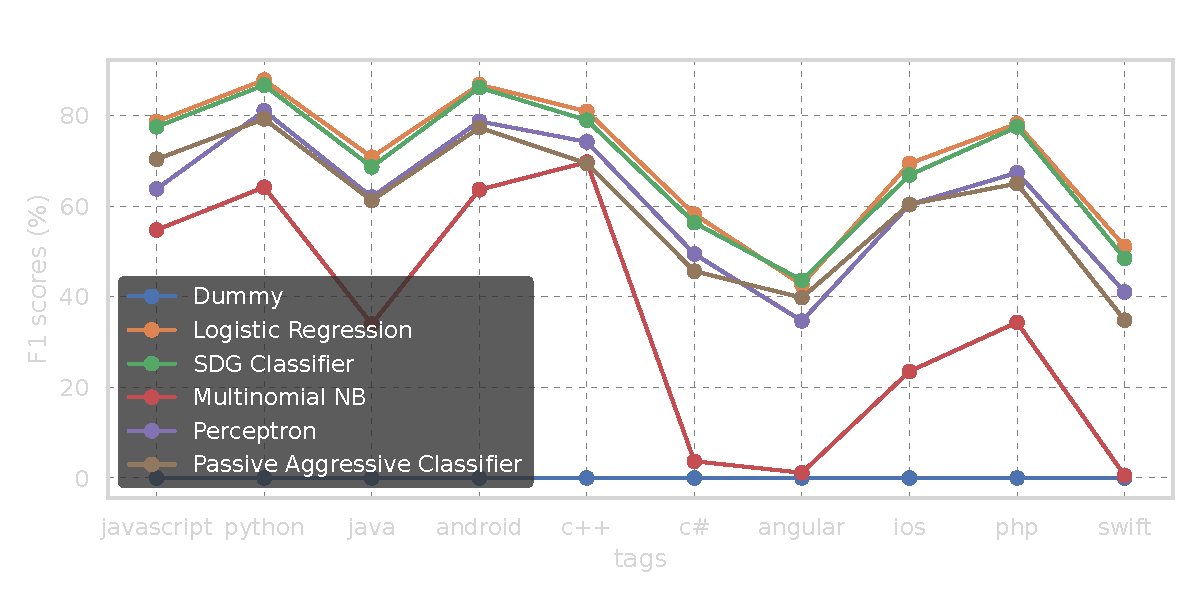
\includegraphics[width=90mm]{F1_scores_models.pdf}} ;

		\onlystyle<4->{shd2}{myShaded}
		\node<3->[shd2] at (\midX,17mm) {La \alert{régression logistique} fourni les \alert{meilleurs résultats}} ;
		\node<4->[text width=70mm, text centered] 
			at (\midX,8mm) {Le \alert{classifieur SGD} est \alert{plus rapide} à entrainer pour des \alert{résultats proches} (temps divisé par 1,4)} ;

	\end{tikzpicture}
\end{frame}


\subsection{Intérêt d'un PCA ?}
\begin{frame}[t, label=PCA]
	\vspace{0mm}
	\begin{tikzpicture}
		\linespread{1}% <--- locally defined vertical line spacing in nodes
		\draw[clrBorders] (0,0) rectangle (\txw,\txh) ;
		\nodePageNumber

		\onlystyle<2->{shd1}{myShaded}
		\node[shd1, text width=40mm, text centered] at (\midX,80mm) {Encodeur : TFIDF (1000 mots)\\modèle : regression logistique} ;

		\node<2> at (\midX,\midY) {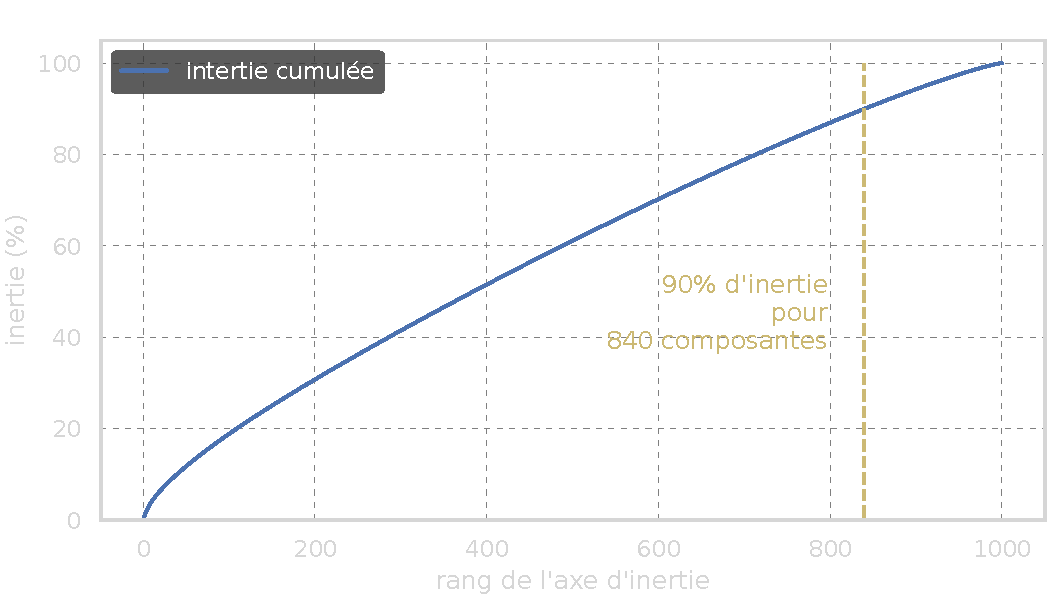
\includegraphics[width=90mm]{ebouli_tfidf.pdf}} ;
		\node<3-> at (\midX,\midY) {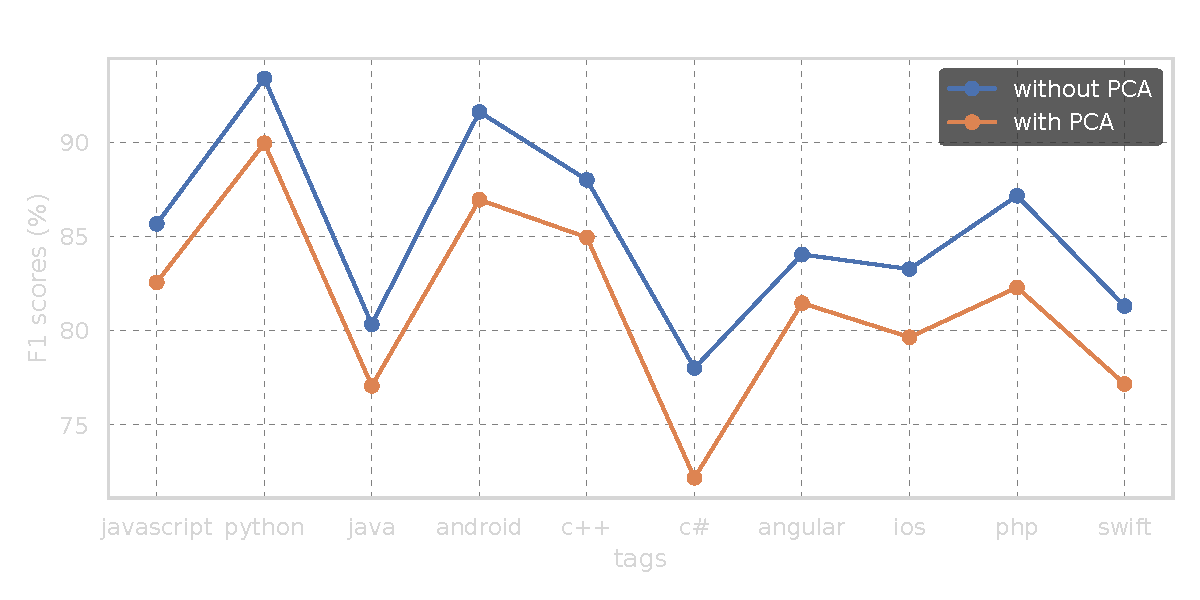
\includegraphics[width=90mm]{F1_scores_PCA.pdf}} ;

		\node<4>[myOrng] at (\midX,15mm) {PCA non pertinente ici} ;
	\end{tikzpicture}
\end{frame}


\subsection{Intérêt d'une régularisation ?}
\begin{frame}[t, label=Régularisation]
	\vspace{0mm}
	\begin{tikzpicture}
		\linespread{1}% <--- locally defined vertical line spacing in nodes
		\draw[clrBorders] (0,0) rectangle (\txw,\txh) ;
		\nodePageNumber

		\onlystyle<2->{shd1}{myShaded}
		\node[shd1, text width=40mm, text centered] at (\midX,80mm) {Encodeur : TFIDF (900 mots)\\modèle : regression logistique} ;
		\node<2-> at (\midX,\midY) {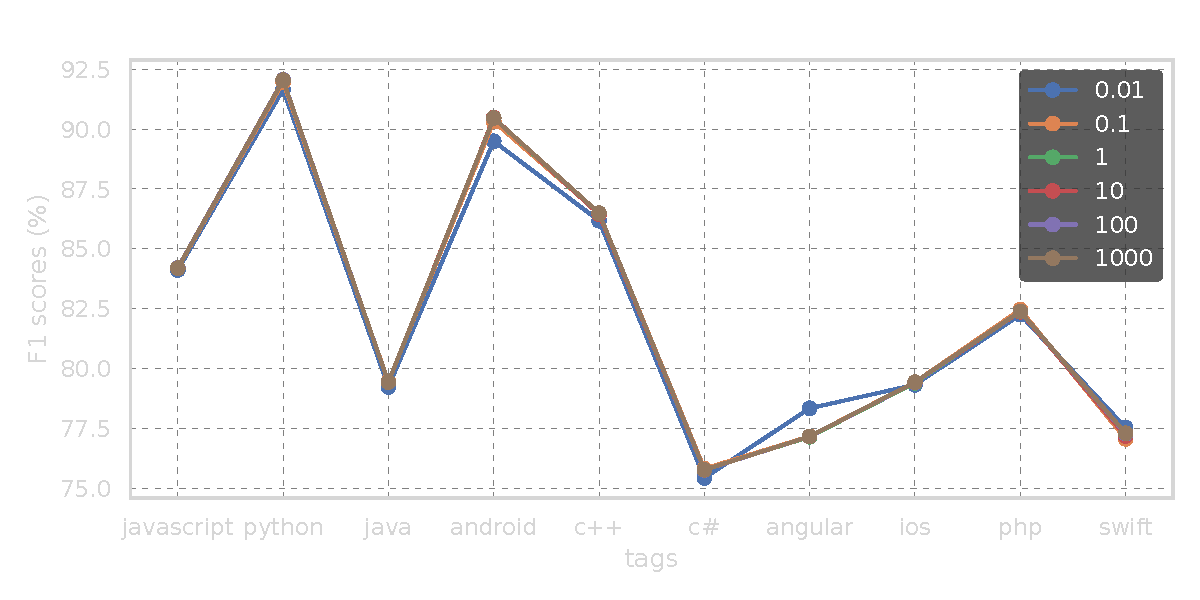
\includegraphics[width=90mm]{F1_scores_regularisation.pdf}} ;

		\node<3> at (\midX,15mm) {\alert{Influence faible} sur les résultats} ;
	\end{tikzpicture}
\end{frame}




\subsection{Longueur du vocabulaire ?}
\begin{frame}[t, label=vocabLength]
	\vspace{0mm}
	\begin{tikzpicture}
		\linespread{1}% <--- locally defined vertical line spacing in nodes
		\draw[clrBorders] (0,0) rectangle (\txw,\txh) ;
		\nodePageNumber

		\onlystyle<2->{shd1}{myShaded}
		\node[shd1, text width=40mm, text centered] at (\midX,80mm) {Encodeur : TFIDF\\modèle : regression logistique} ;
		\node<2-> at (\midX,\midY) {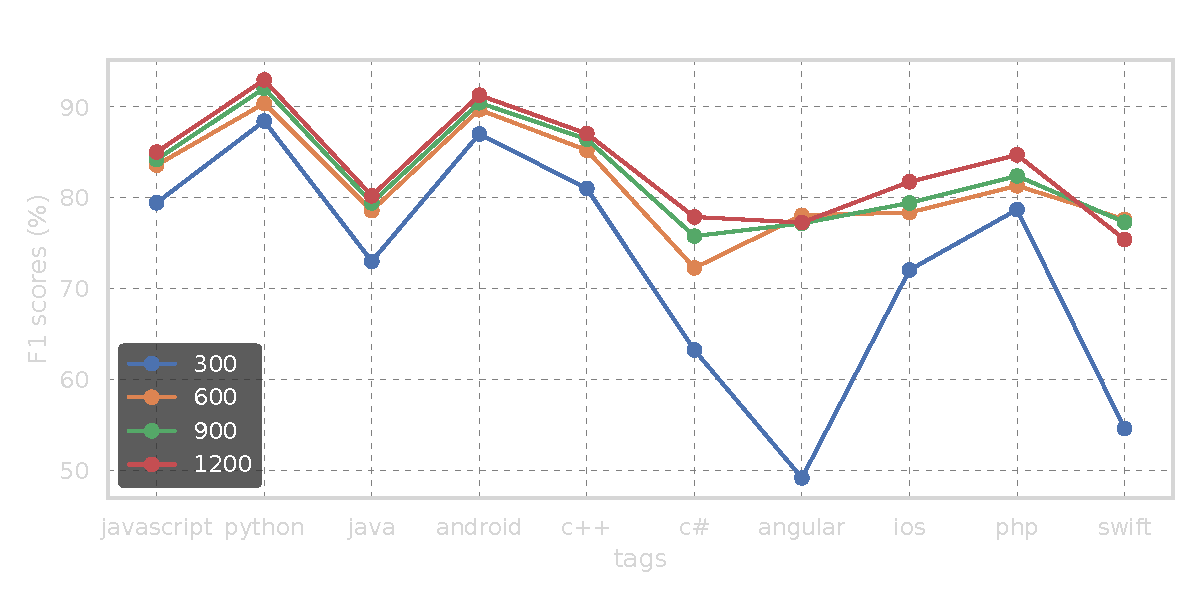
\includegraphics[width=90mm]{F1_scores_vocab_length.pdf}} ;

		\node<3>[myOrng] at (\midX,15mm) {Influence variable selon les tags} ;
	\end{tikzpicture}
\end{frame}



\subsection{Optimisation du seuil de décision}
\begin{frame}[t, label=OptimThreshold]
	\vspace{0mm}
	\begin{tikzpicture}
		\linespread{1}% <--- locally defined vertical line spacing in nodes
		\draw[clrBorders] (0,0) rectangle (\txw,\txh) ;
		\nodePageNumber

		\onlystyle<2->{shd1}{myShaded}
		\node[shd1] at (\midX,80mm) {Optimisation du seuil de décision par tag} ;
		\node<2-> at (\midX,\midY) {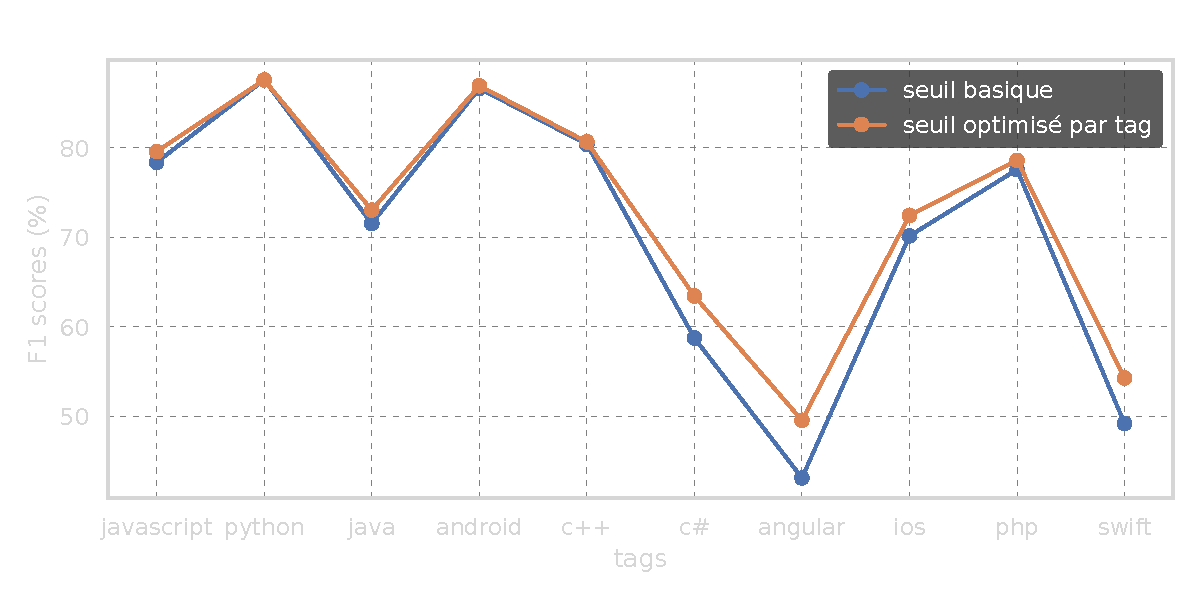
\includegraphics[width=90mm]{F1_scores_decision_threshold.pdf}} ;

		\node<3-> at (\midX,15mm) {\alert{Amélioration intéressante} pour les scores les plus bas} ;
	\end{tikzpicture}
\end{frame}



\subsection{Quel encodeur ?}
\begin{frame}[t, label=Encodeurs]
	\vspace{0mm}
	\begin{tikzpicture}
		\linespread{1}% <--- locally defined vertical line spacing in nodes
		\draw[clrBorders] (0,0) rectangle (\txw,\txh) ;
		\nodePageNumber

		\onlystyle<2->{shd1}{myShaded}
		\node[shd1] at (\midX,80mm) {Différents encodeurs} ;

		\onlystyle<3->{shd2}{myShaded}
		\begin{scope}[xshift=\midX-15mm, yshift=75mm]
			\node<2-8>[shd2] at (0,-5mm) {Méthodes explorées:} ;
			\foreach[count=\i, evaluate=\i as \ii using int(\i+2)] \x in {TFIDF (900 mots), Word2Vec, Sentence BERT, Universal Sentence Encoder}
			{
				\node<\ii-8>[box_style00] at (0,-\i*12mm-5mm) {\x} ;
			}
			\draw<7-8>[box_style00, thick, myOrng] (0-15mm, -17mm-5mm) rectangle (0+15mm, -17mm+5mm) ;
			\onlystyle<8->{shd2}{myShaded}
			\node<7-8>[shd2] at (35mm, -17mm) {approche \alert{bag-of-word}} ;
			\draw<8>[box_style00, thick, myOrng] (0-21mm, -41mm-17mm) rectangle (0+21mm, -41mm+17mm) ;
			\node<8>[text centered, text width=40mm] at (42mm, -41mm) {approche\\\alert{word/sentence embedding}} ;
		\end{scope}

		\node<9-> at (\midX,\midY) {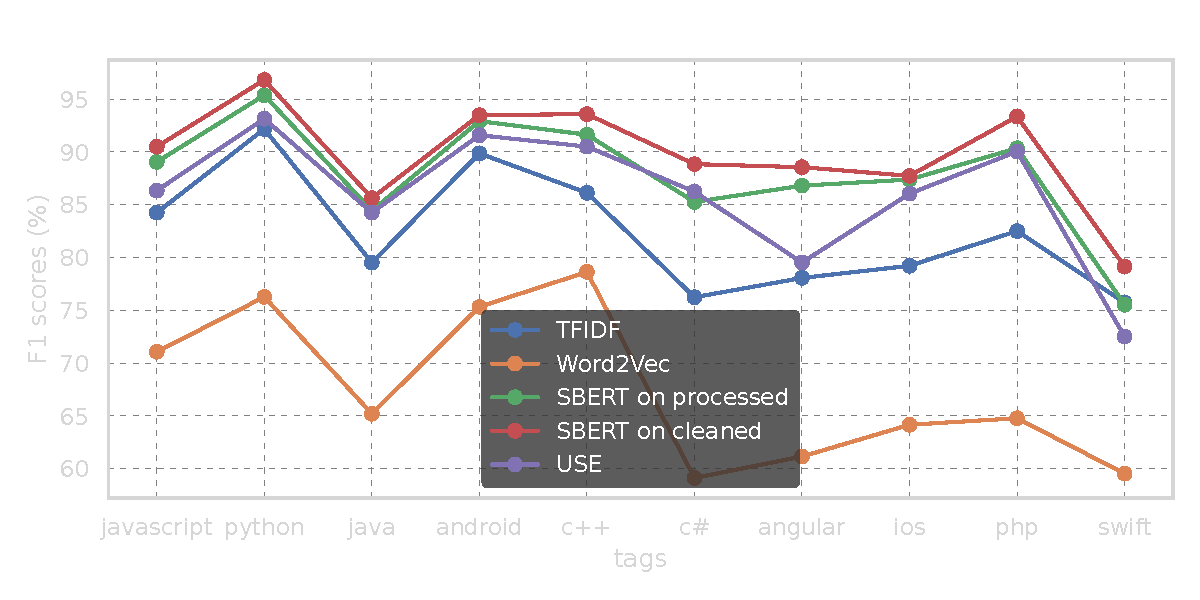
\includegraphics[width=90mm]{F1_scores_vectorizer.pdf}} ;
		\node<10> at (\midX,15mm) {Les \alert{meilleurs résultats} sont obtenus avec \alert{Sentence BERT} } ;
	\end{tikzpicture}
\end{frame}



\subsection{Conclusions}
\begin{frame}[t, label=EssaisCCL]
	\vspace{0mm}
	\begin{tikzpicture}
		\linespread{1}% <--- locally defined vertical line spacing in nodes
		\draw[clrBorders] (0,0) rectangle (\txw,\txh) ;
		\nodePageNumber

		\onlystyle<2->{shd1}{myShaded}
		\node[shd1] at (\midX,80mm) {Conclusions des essais} ;

		\onlystyle<3->{shd2}{myShaded}
		\node<2->[box_style00, text width=62mm, shd2] at (\midX,65mm) {La \alert{PCA} semble \alert{non appropriée} pour ce projet} ;
		
		\onlystyle<4->{shd3}{myShaded}
		\node<3->[box_style00, text width=62mm, shd3] at (\midX,45mm) {L'encodeur \alert{Sentence BERT} est choisi} ;
		
		\node<4->[box_style00, text width=62mm] at (\midX,25mm) {La \alert{régression logistique} est sélectionnée comme classifieur} ;
	\end{tikzpicture}
\end{frame}


\section{API}
\begin{frame}[t, label=APIdemo]
	\vspace{0mm}
	\begin{tikzpicture}
		\linespread{1}% <--- locally defined vertical line spacing in nodes
		\draw[clrBorders] (0,0) rectangle (\txw,\txh) ;
		\nodePageNumber

		\onlystyle<2->{shd1}{myShaded}
		\node[shd1] at (\midX,80mm) {Interface de programmation d'application (API)} ;

		\onlystyle<3->{shd2}{myShaded}
		\node<2->[box_style00,shd2] at (\midX,70mm) {API servie sous \alert{flask}} ;
		\onlystyle<4->{shd3}{myShaded}
		\node<3->[box_style00,shd3] at (\midX,55mm) {Sur un \alert{serveur AWS}} ;
		\onlystyle<5->{shd4}{myShaded}
		\node<4->[box_style00,shd4] at (\midX,40mm) {En utilisant \alert{gunicorn}} ;
		
		\node<5>[box_style00] at (\midX,20mm) {Démonstration} ;

	\end{tikzpicture}
\end{frame}

\section{CONCLUSIONS}

\begin{frame}[t, label=CCL]
	\vspace{0mm}
	\begin{tikzpicture}
		\linespread{1}% <--- locally defined vertical line spacing in nodes
		\draw[clrBorders] (0,0) rectangle (\txw,\txh) ;
		\nodePageNumber

		\onlystyle<2->{shd1}{myShaded}
		\node[box_style00,shd1] at (\midX,70mm) {Découverte de la \alert{gestion} des \alert{données textuelles}} ;
		\onlystyle<3->{shd2}{myShaded}
		\node<2->[box_style00, text width=60mm, shd2] at (\midX,55mm)
		{Sélection de la meilleur solution:\\\alert{Sentence BERT} + \alert{régression logistique}} ;
		\onlystyle<4->{shd3}{myShaded}
		\node<3->[box_style00, text width=60mm, shd3] at (\midX,40mm) {Développement d'une\\\alert{interface de programmation d'application}} ;
		\node<4>[box_style00] at (\midX,25mm) {\alert{Déployement} de l'\alert{interface} sur un \alert{serveur AWS}} ;

	\end{tikzpicture}
\end{frame}

\section{PERSPECTIVES}

\begin{frame}[t, label=Perspectives]
	\vspace{0mm}
	\begin{tikzpicture}
		\linespread{1}% <--- locally defined vertical line spacing in nodes
		\draw[clrBorders] (0,0) rectangle (\txw,\txh) ;
		\nodePageNumber

		\onlystyle<2->{shd1}{myShaded}
		\node[box_style00,shd1] at (\midX,70mm) {Entrainer un \alert{ExtraTrees} sur un \alert{serveur}} ;
		\onlystyle<3->{shd2}{myShaded}
		\node<2->[box_style00, text width=60mm, shd2] at (\midX,55mm)
		{Entrainer le modèle à prédir \alert{plus de tags}} ;
		% \onlystyle<4->{shd3}{myShaded}
		\node<3->[box_style00, text width=60mm] at (\midX,40mm)
			{\alert{Déployement} de l'interface sécurisé $\rightarrow$ \alert{https}} ;
		% \node<4>[box_style00] at (\midX,25mm) {\alert{Déployement} de l'\alert{interface} sur un \alert{serveur AWS}} ;

	\end{tikzpicture}
\end{frame}


\begin{frame}[t, label=Merci]
	\vspace{0mm}
	\begin{tikzpicture}
		\linespread{1}% <--- locally defined vertical line spacing in nodes
		\draw[clrBorders] (0,0) rectangle (\textwidth,\textheight) ;

		\node at (0.5\textwidth,\midY) {\huge \alert{Merci} pour votre \alert{attention}.} ;

	\end{tikzpicture}
\end{frame}


\end{document}
